\chapter{Test of Antenna Characteristics}
\section{Test of Horn Antenna S-Parameters} \label{s:sparam_test}
The aim of this test is to find $S_{11}$ and the reflection coefficient of the receiving antenna. The measurement will be used to choose the resonance frequency for the acceptance test.

\subsection{Equipment}
To perform the test the following equipment is needed:
\begin{itemize}
    \item Rohde \& Schwarz ZNA Vector Network Analyzer (\SI{10}{\mega\hertz}-\SI{43.5}{\giga\hertz})
    \item Rohde \& Schwarz ZN-Z54 Calibration Unit (\SI{9}{\kilo\hertz}-\SI{40}{\giga\hertz})
    \item \SI{50}{\ohm} antenna cable
    \item DUT - horn antenna
\end{itemize}

\subsection{Procedure}
The test is performed once. The following explains the procedure for the test:
\begin{enumerate}
    \item Add power to VNA, connect antenna cable to VNA and Calibration unit.
    \item Make calibration test by choosing \textit{Cal $\rightarrow$ Quick Start Calibration $\rightarrow$ Apply} on the VNA.
    \item Disconnect antenna cable and reconnect to DUT.
    \item Set start and stop frequencies. 
    \item Ensure that VNA measures $S_{11}$-parameter by choosing \textit{Meas $\rightarrow$ $S_{11}$}.
\end{enumerate}
The antennas are identical horn antennas which are designed to work in the spectrum from \SI{4}{\giga\hertz} to \SI{7}{\giga\hertz}. The measurement is performed in the spectrum \SI{3}{\giga\hertz} to \SI{8}{\giga\hertz} in order to encapsulate the entire antenna frequency spectrum, with steps of \SI{25}{\mega\hertz}. 

\subsection{Result}
The following figure shows $S_{11}$ as a function of frequency. The criterion considered for impedance matching is a reflection coefficient of \SI{-10}{\decibel}. In order to perform the measurements, the two resonance frequencies (\SI{4.75}{\giga\hertz} and \SI{5.65}{\giga\hertz}) have been chosen.
\begin{figure}[H]
    \centering
    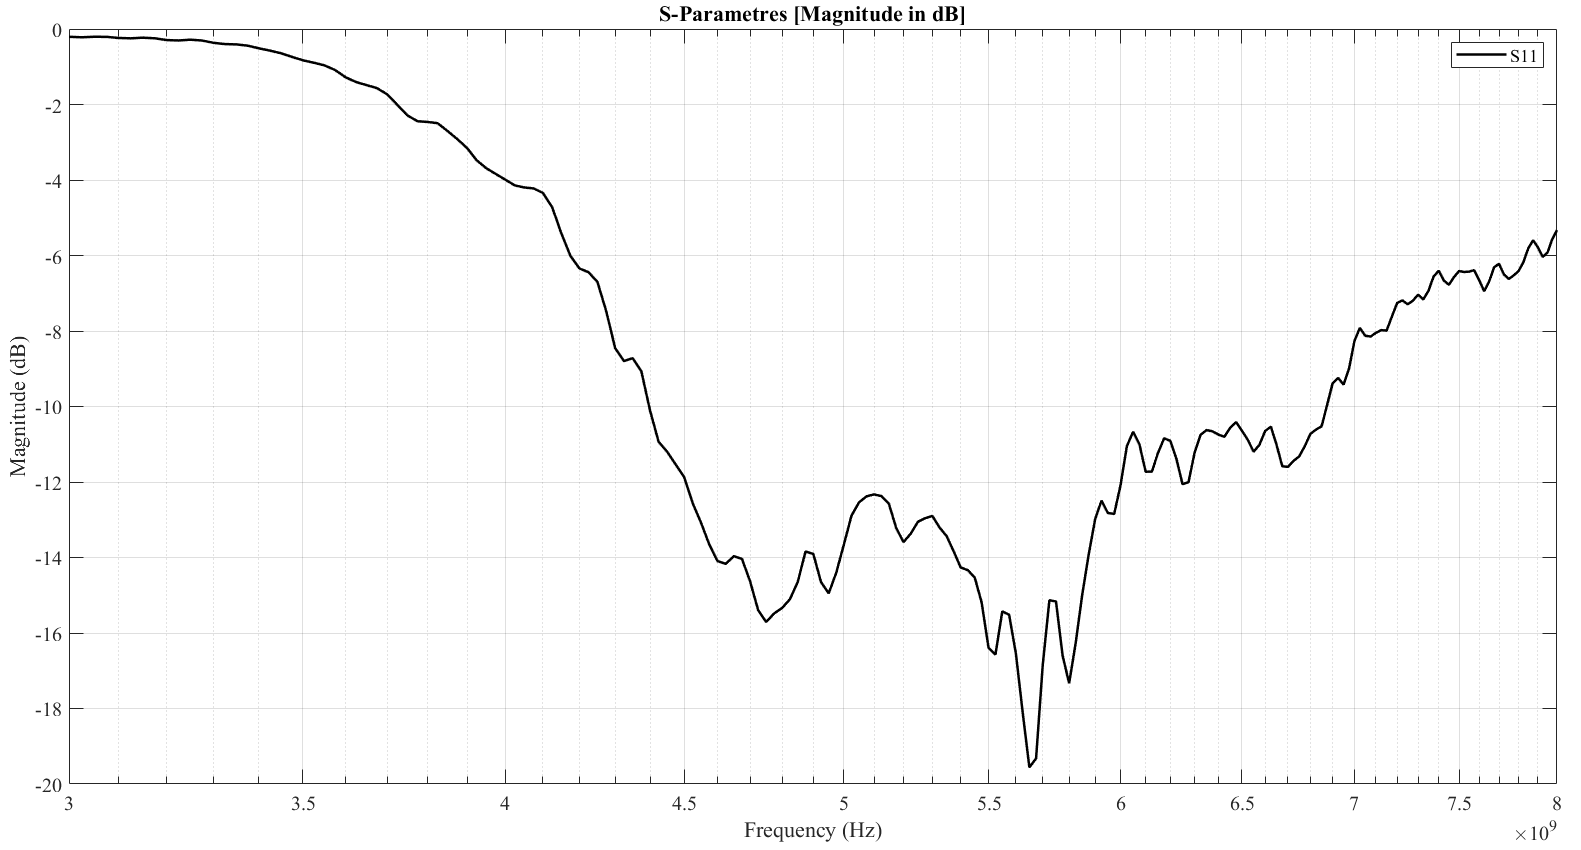
\includegraphics[width=1\textwidth]{figures/s11_meas.png}
    \caption{Measured $S_{11}$-parameter from \SI{3}{\giga\hertz} to \SI{8}{\giga\hertz}.} \label{fig:s11_meas}
\end{figure}
It can be seen that the antenna has a maximum $S_{11}$ magnitude of \SI{-19.56}{\decibel} at \SI{5.65}{\giga\hertz}. This gives a reflection coefficient of $\Gamma = 10^{-19.56/20} = 0.11$. Almost \SI{1}{\giga\hertz} away at \SI{4.75}{\giga\hertz} the magnitude of $S_{11}$ is \SI{-15.71}{\decibel} which equals a reflection coefficient of $\Gamma = 10^{-15.71/20} = 0.16$.

\section{Test of Horn Antenna Radiation Pattern} \label{s:rad_test}
The aim of this test is to know the directiveness of the antennas to obtain the \SI{3}{\decibel} bandwidth of the antennas and determine the step angle needed in the turntable.

\subsection{Equipment}
The test is performed in the anechoic chamber at Aalborg University with the provided setup equipment at the site. This includes:
\begin{itemize}
    \item Computer with relevant \textit{MVG software}
    \item \textit{MVG StarMIMO} in anechoic chamber
\end{itemize}
The \textit{MVG StarMIMO} has a measurement bandwidth of \SI{400}{\mega\hertz} to \SI{6}{\giga\hertz}. As seen in the results in the test of S-parameters in subsection \ref{s:sparam_test} the maximum reflection coefficient magnitude is at \SI{5.65}{\giga\hertz}, therefore the step size of frequency spectrum for the radiation characteristics measurement is chosen to be \SI{0.05}{\giga\hertz}.

\subsection{Procedure}
The following explains the procedure for the test:
\begin{enumerate}
    \item Measure known antenna \textit{(MVG SH800)} with known radiation characteristics. Use for gain reference.
    \item Secure DUT to test platform.
    \item Perform automated test by activating the measurement equipment of the chamber.
\end{enumerate}
Since the antenna is not designed for use below \SI{4}{\giga\hertz}, this is set as the start frequency. The measurement equipment cannot measure above \SI{6}{\giga\hertz}, therefore this is the end frequency. The StarMIMO measures at angle steps of \SI{15}{\degree} in both planes.

\subsection{Result}
The data collected is imported into \textit{Matlab} for visualization. The figure \ref{fig:horn_elevation} shows the elevation plane of the measured horn antenna in the anechoic chamber. The red line shows the radiation pattern for the horn antenna at $f=\SI{4.75}{\giga\hertz}$. The blue line shows the radiation pattern for the horn antenna at $f=\SI{5.65}{\giga\hertz}$. The antenna has a higher gain at $f=\SI{5.65}{\giga\hertz}$ of \SI{12.99}{\decibel}, whereas at $f=\SI{4.75}{\giga\hertz}$ the highest gain is \SI{11.41}{\decibel}. The \SI{3}{\decibel}-bandwidths are also plotted at \SI{19}{\degree} for $f=\SI{5.65}{\giga\hertz}$ and at \SI{22.5}{\degree} for $f=\SI{4.75}{\giga\hertz}$. For this reason, the chosen angle step for the measurements with the turntable is \SI{20}{\degree}.
\begin{figure}[H]
    \centering
    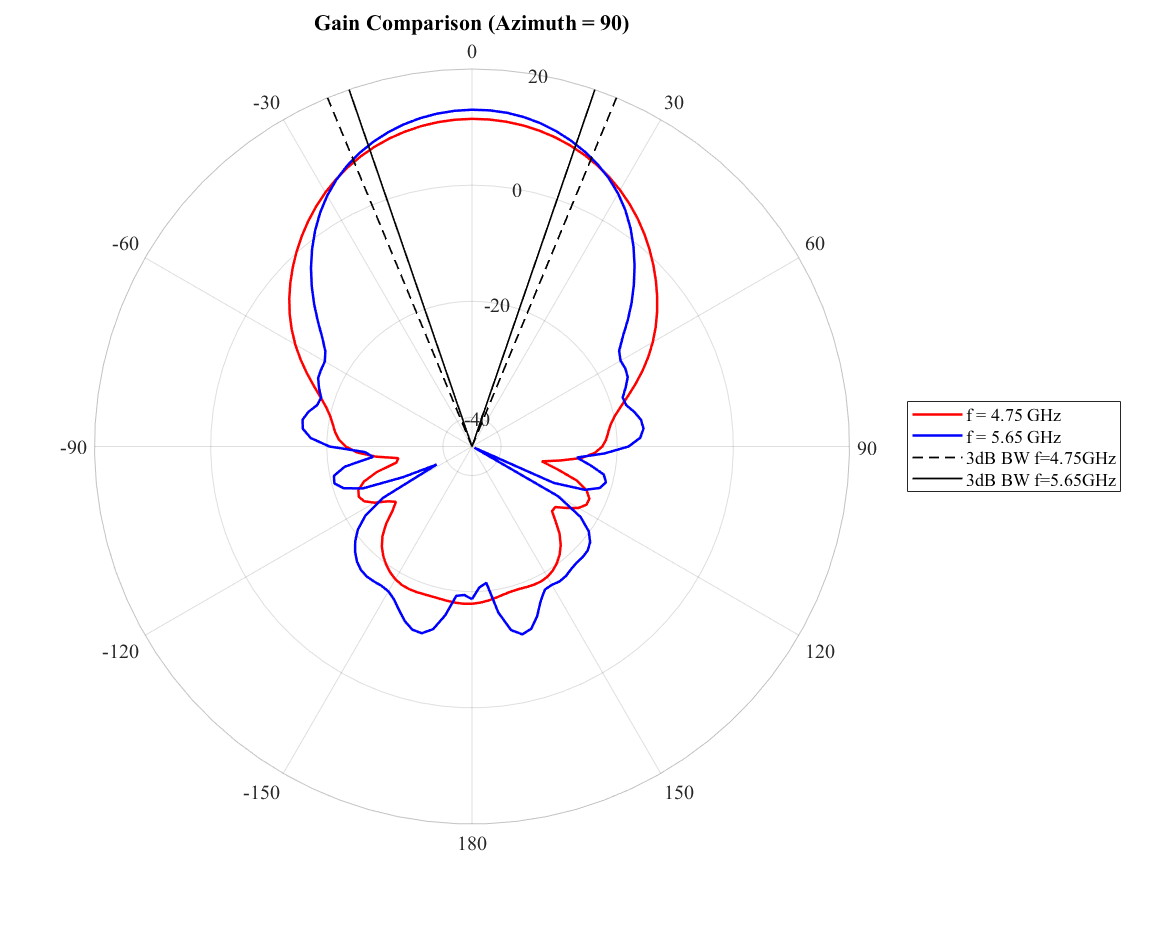
\includegraphics[width=1\textwidth]{figures/horn_elevation.png}
    \caption{Measured gain in the farfield at \SI{4.75}{\giga\hertz} and \SI{5.65}{\giga\hertz} (elevation plane).} 
    \label{fig:horn_elevation}
\end{figure}

Figure \ref{fig:horn_azimuth} shows the azimuth plane of the horn antenna as measured in the anechoic chamber. The red line shows the gain for the antenna at $f=\SI{4.75}{\giga\hertz}$ and the blue line shows the gain for the antenna at $f=\SI{5.65}{\giga\hertz}$. The maximum gain is \SI{12.99}{\decibel} at \SI{0}{\degree}. 
\begin{figure}[H]
    \centering
    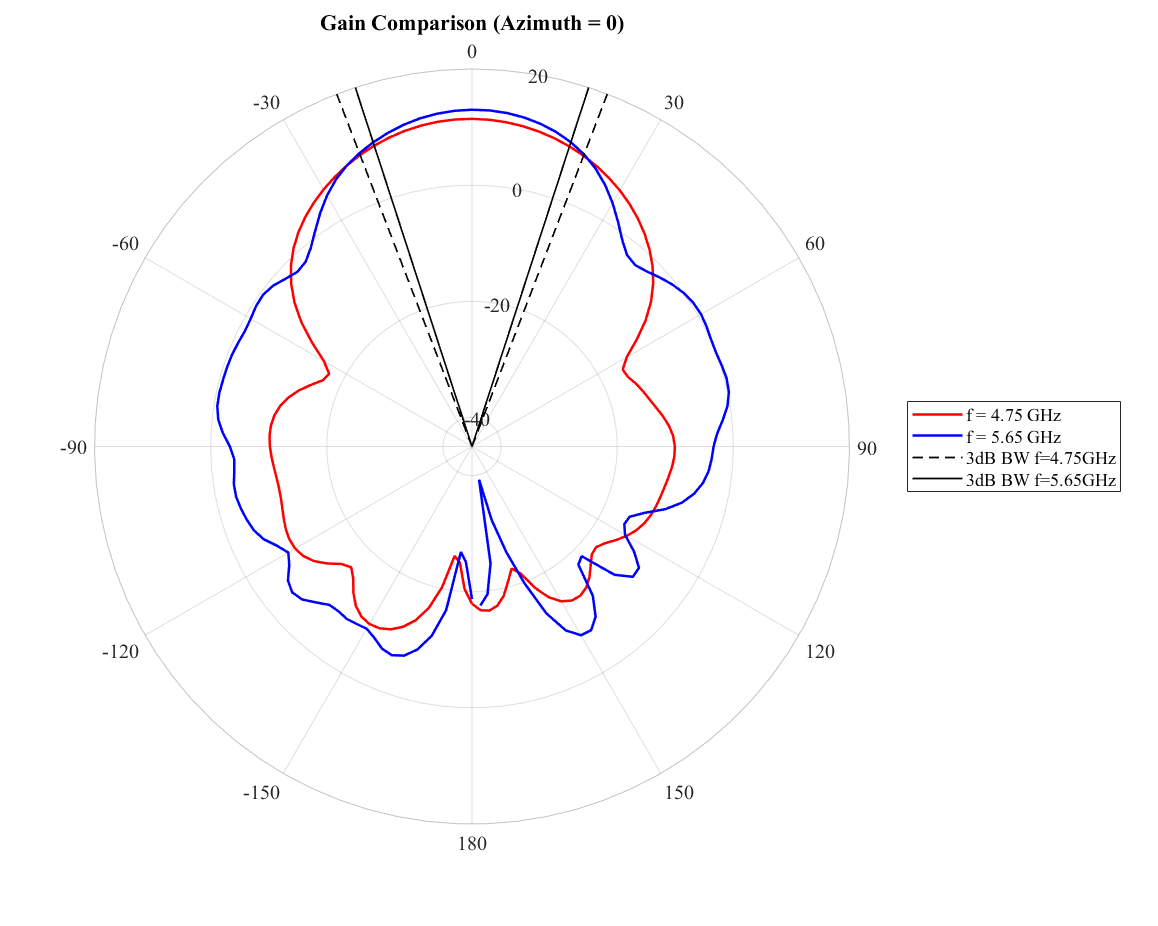
\includegraphics[width=1\textwidth]{figures/horn_azimuth.png}
    \caption{Measured gain in the farfield at \SI{4.75}{\giga\hertz} and \SI{5.65}{\giga\hertz} (azimuth plane).} 
    \label{fig:horn_azimuth}
\end{figure}

The evolution of the gain in the boresight direction as a function of frequency is plotted in figure \ref{fig:gain_meas}. The measurement shows that the gain, generally, increases as the frequency increases.
\begin{figure}[H]
    \centering
    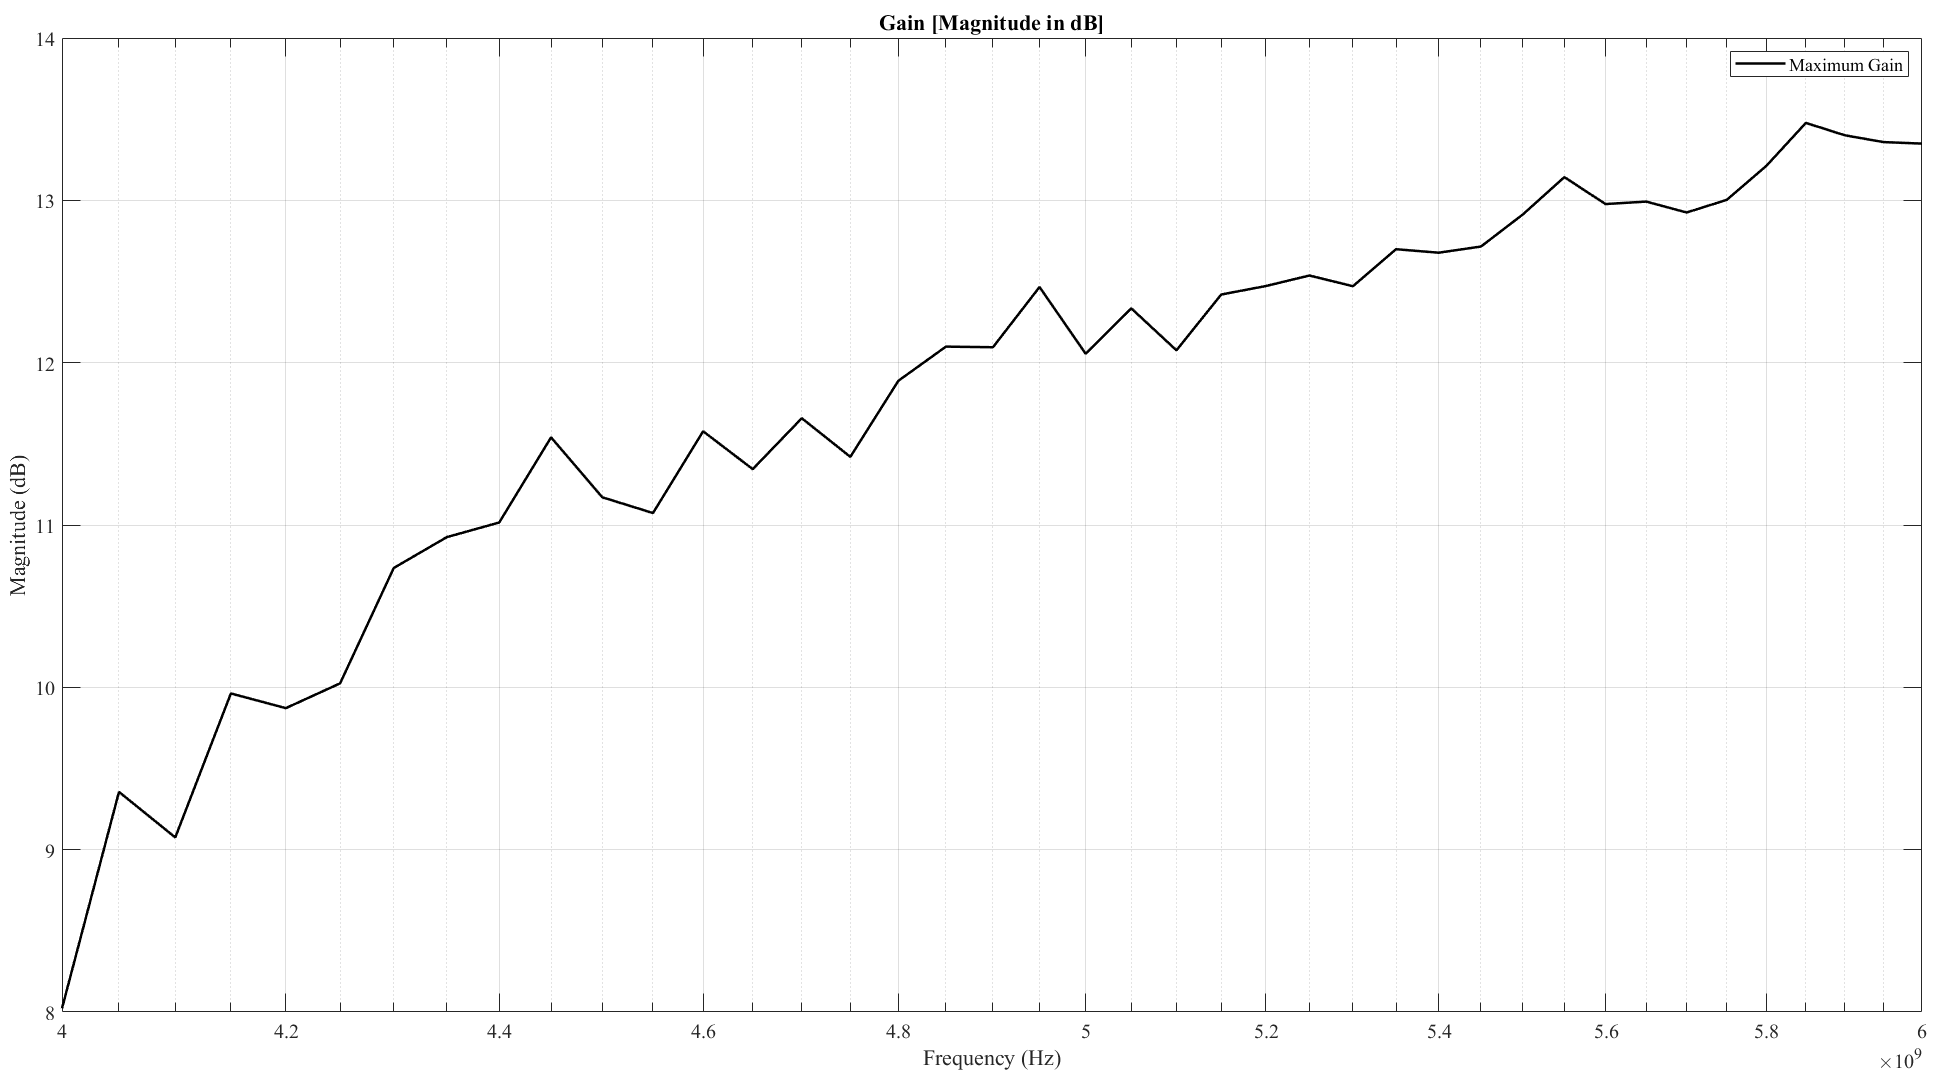
\includegraphics[width=1\textwidth]{figures/gain_meas.png}
    \caption{Measured gain of horn antenna in the boresight direction in the frequency spectrum from \SI{4}{\giga\hertz} to \SI{6}{\giga\hertz}.} \label{fig:gain_meas}
\end{figure}